\documentclass[11pt,a4paper]{article}
\usepackage{fontspec}
\usepackage{xunicode}
\usepackage{xeCJK}
\usepackage{geometry}
\geometry{left=2.5cm, right=2.5cm, top=2.5cm, bottom=2.5cm}

\usepackage{graphicx}
\usepackage{float}
\usepackage{amsmath}
\usepackage{listings}
\lstset{
  language={},
  %numbers=left,
	frame=shadowbox,
	xleftmargin=6mm,
	xrightmargin=2mm,
	basicstyle={\linespread{0.9}\footnotesize\ttfamily}
}

\usepackage{appendix}

\setmainfont{CMU Serif}
\setsansfont{CMU Serif}
\setmonofont{CMU Typewriter Text}

\setCJKmainfont{SimSun}
\setCJKsansfont{SimSun}
\setCJKmonofont{SimSun}

\usepackage{datetime}
\renewcommand{\today}{\number\year 年 \number\month 月 \number\day 日}
%\renewcommand{\abstractname}{}
%\renewcommand{\contentsname}{}

\title{``基于NI myDAQ的自动控制原理实验套件''设计说明}


\begin{document}
\author{自动控制原理实验室}

\maketitle

\begin{abstract}
  本项目以MATLAB/Simulink为实验环境,将National Instruments公司出品的myDAQ可编程测量设备作为模拟/数字接口,使计算机与外部硬件交互,进而设计了用于自动控制原理教学实验的三套实验设备。每个实验所需的硬件以一块板卡的形式与myDAQ连接,并可与MATLAB中的软件控制器或虚拟受控对象交互。通过更换板卡,学生可选择进行不同的实验。
\end{abstract}

\tableofcontents

\section{NI myDAQ 接线端子适配器}

\subsection{设计目的}
NI myDAQ可编程测量设备的右侧带有20个螺丝接线端子,原本被设计用于接入单根导线,可为原型实验板上的项目供电,并通过模拟数字I/O通道读取数据。在此项目中myDAQ将与固定的数个实验板卡连接,且实验板卡需要经常更换,因此需要设计一种适配器板卡,将螺丝接线端子转换为易于插拔的连接器。

\subsection{连接器选型}
考虑到设备由经验不一定丰富的学生进行操作,用于与实验板卡对接的连接器需要满足以下要求:
\begin{enumerate}
\item 连接器或线缆至少可以承载20路信号,其中包含5V/15V供电线路。
\item 具有良好的防呆(防止接反、接错位)特性;
\item 需要足够牢固,具有良好的机械性能;
\item 使用寿命足够长。
\end{enumerate}

最初考虑的是使用2.54mm间距的排针与排座进行对接。但是这种方法十分容易被连接错位,并且机械强度不够高。之后考虑了在转接器和实验板卡之间使用线缆连接。USB Type-C连接器在区分正反插的条件下可以承载20路信号,但是这种连接器和线缆成本高且不易买到。最终使用的是D-Sub 25针连接器。连接器可被焊在转接器右侧和实验板卡左侧,可以直接对接,也可以使用线缆连接。插座周围有金属外壳,可以防止接反和接错位。

\subsection{硬件与PCB设计}
转接器上除了包含必要的电源滤波、退耦电路外,设计了300mA自恢复保险丝来提供额外电气保护。myDAQ设备上只有一个蓝色指示灯,当USB设备枚举成功时会点亮。转接器上为$\pm$15V模拟组件电源、5V数字组件电源预留了指示灯。如出现电源电流过大的情况,myDAQ自动关闭电源或自恢复保险丝断路,指示灯熄灭,可帮助及时发现故障。

\begin{figure}[h!]\centering
  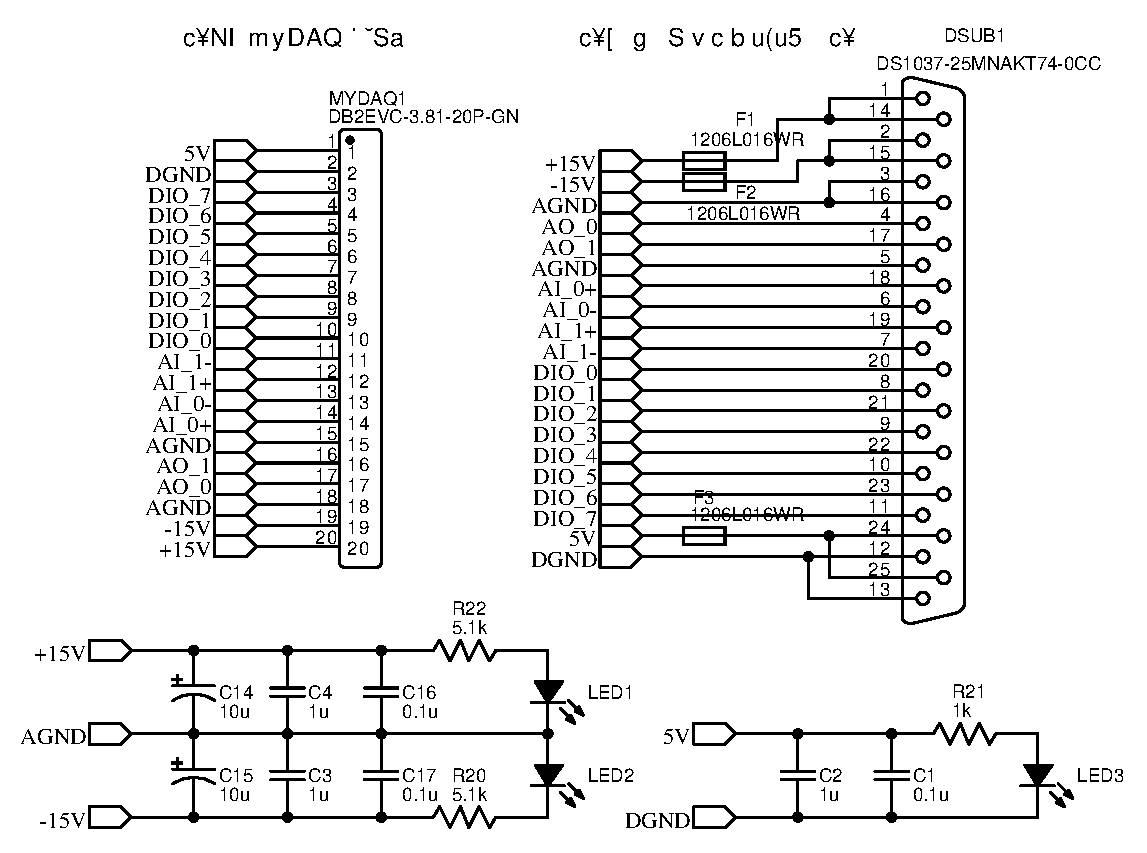
\includegraphics[width=12cm]{./figs/conv_sch.pdf}
  \caption{myDAQ接线端子适配器的原理图}\label{conv_sch}
\end{figure}

\begin{figure}[h!]\centering
  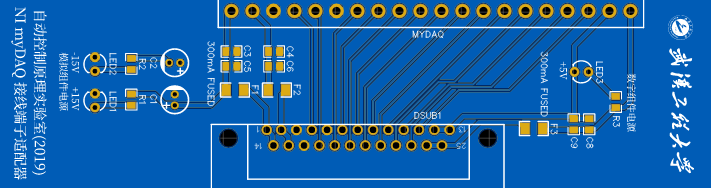
\includegraphics[width=13cm]{./figs/conv_pcb.png}
  \caption{myDAQ接线端子适配器的PCB设计图}\label{conv_pcb}
\end{figure}


\section{模拟电路比例-积分-微分(PID)控制器}

\subsection{设计目的}
板卡上设计了基于运算放大器的PID调节器电路。myDAQ以模拟电压的形式给出一个误差量,电路将通过其比例-积分-微分环节输出一个调节量,并反馈到myDAQ的模拟输入通道中。在Simulink环境中以离散传递函数的形式建立一个虚拟对象,例如一个虚拟直流电机,并使此对象接受硬件PID调节器的控制。学生可使用拨码开关设置PID调节器的参数,使用虚拟示波器等Simulink中的工具观察PID调节器与受控对象的状态。

\subsection{PID调节器与硬件设计}
图\ref{pid_sch}为PID调节器的原理图。SW1 -- SW5为DIP拨码开关,在进行实验时,学生可选择不同参数的电阻或电容接入电路。

\begin{figure}[h!]\centering
  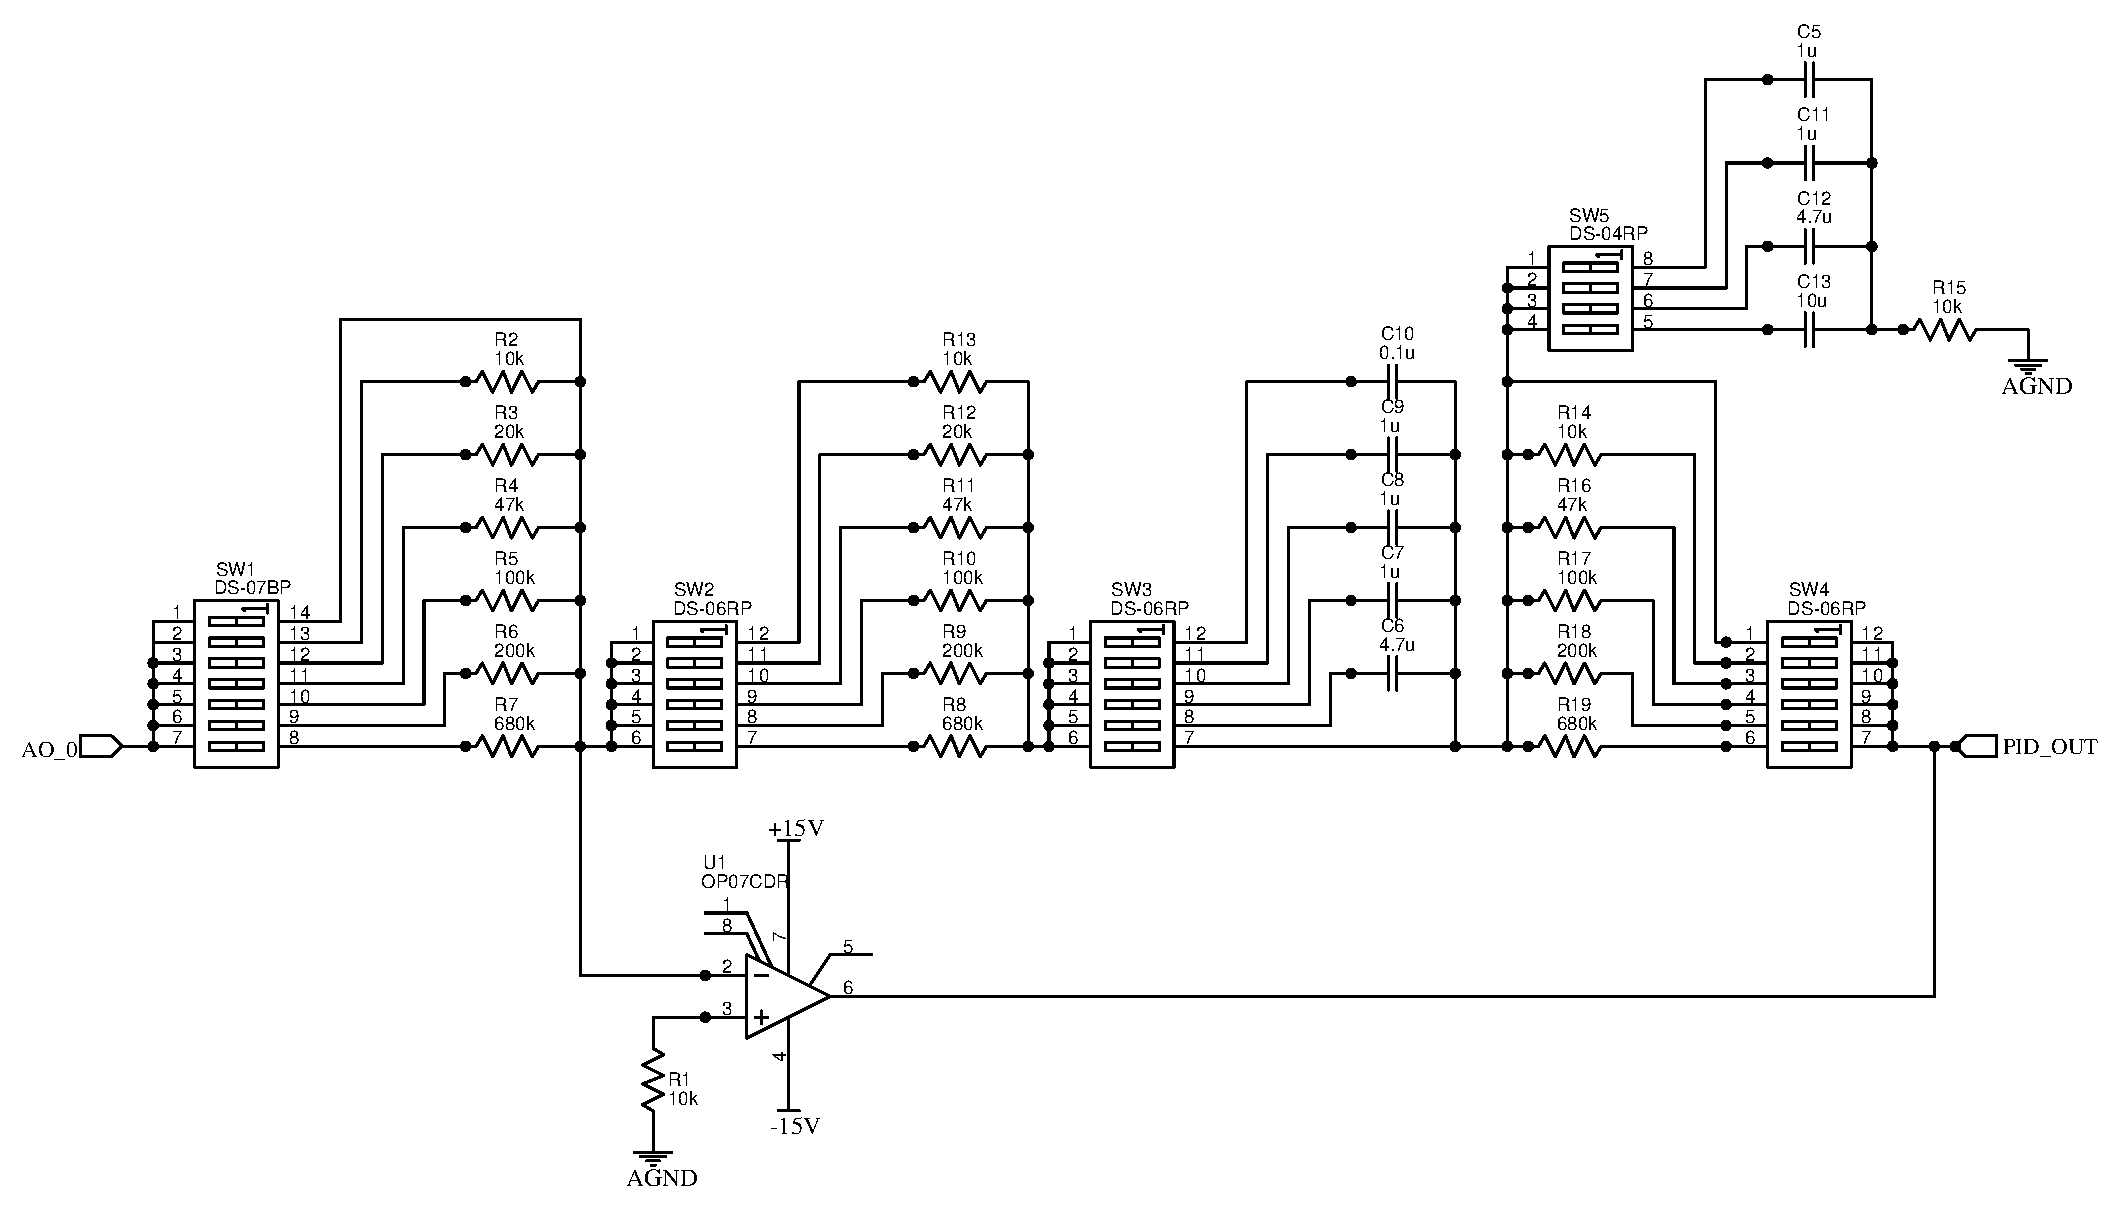
\includegraphics[width=14cm]{./figs/pid_sch.pdf}
  \caption{PID调节器的原理图}\label{pid_sch}
\end{figure}

图\ref{pid_board}为PID实验板卡的设计图。板卡上设计了原理图丝印,并将拨码开关放置于与丝印原理图匹配的位置,方便学生调节和理解。板上设计了用于供电和信号引出的焊盘,可安装2mm香蕉插座。接入外接电源后,板卡脱离myDAQ实验环境也可使用。

\begin{figure}[h!]\centering
  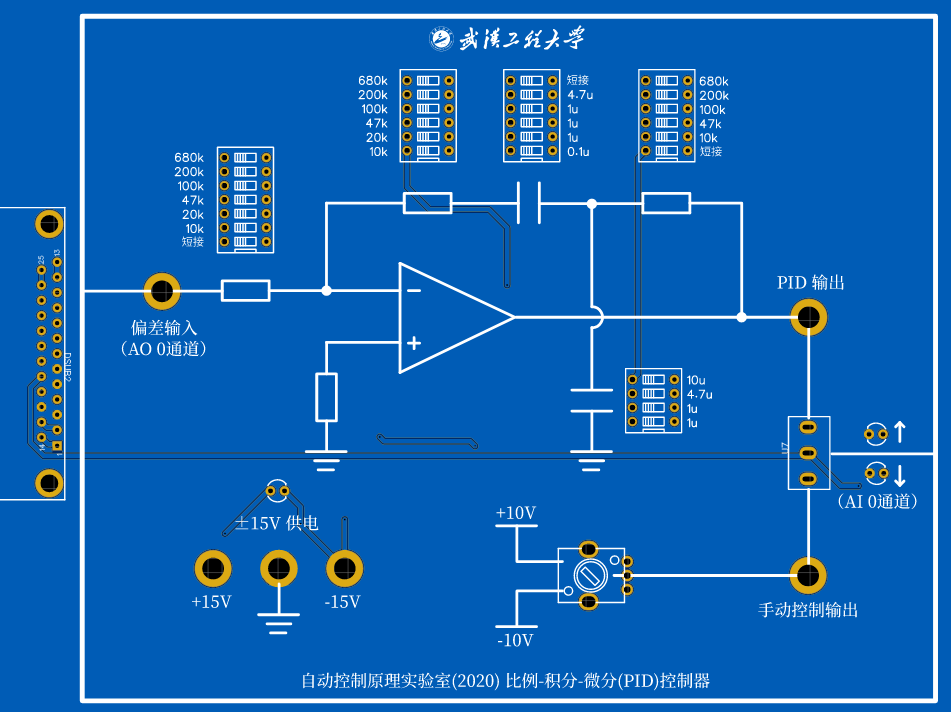
\includegraphics[width=14cm]{./figs/pid_board.png}
  \caption{PID控制器实验PCB设计图}\label{pid_board}
\end{figure}

板上设计了调节器输出指示灯,可用于指示PID调节器正在增加或减少控制量的状态。板上有一个单圈电位器,用于手动输出-10V -- +10V模拟电压接入被控对象。PID和手动模式可使用钮子开关U7进行切换。

\subsection{虚拟对象的Simulink模型}
在Simulink中设计了图\ref{virtual_motor}所示的模型。其中的虚拟对象(电机)以一个二阶离散传递函数表示:
\begin{equation}
  \operatorname{\hat{y}}(k) = \frac{0.3816 \cdot z^{-1}}{1 - 0.4219 \cdot z^{-1} - 0.4749 \cdot z^{-2}} \cdot \operatorname{u}(k)
\end{equation}

\begin{figure}[h!]\centering
  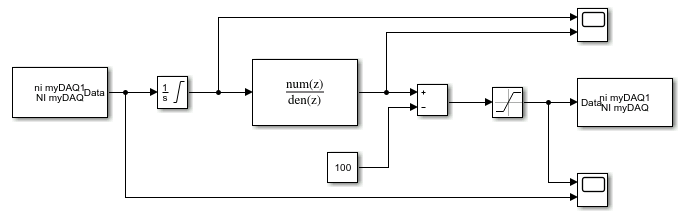
\includegraphics[width=12cm]{./figs/virtual_motor.png}
  \caption{用于实验的Simulink模型}\label{virtual_motor}
\end{figure}

此传递函数是由一个实际直流电机利用系统辨识方法生成的。图\ref{model_response}为在同一激励源下,模型的响应与实际电机的响应。由图可知二阶模型具有良好的拟合效果,并且误差在可接受范围内,可以用于实验。

\begin{figure}[h!]\centering
  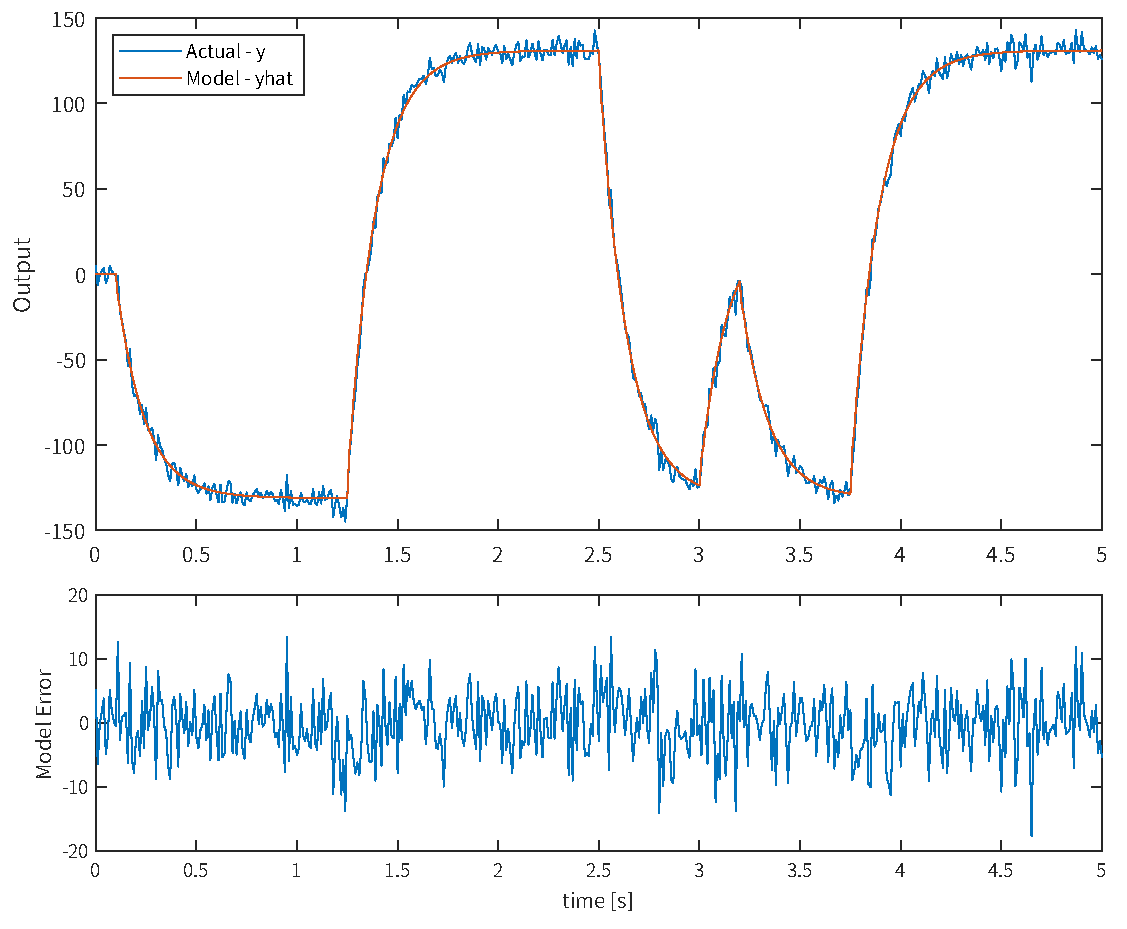
\includegraphics[width=11cm]{./figs/verify_211.pdf}
  \caption{同一激励源下电机响应与二阶传递函数模型响应的比较\label{model_response}}
\end{figure}


\section{直流电机调速实验}

\subsection{设计目的}
板卡上设计了直流电机驱动、转速测量与电流测量电路。myDAQ输出一个0--10V的模拟电压信号来控制板上电机的功率,电机的状态经过光电对管和电流采样电路测量,以0--10V模拟电压的形式送至myDAQ的模拟输入端口上,对应转速测量范围0 -- 10000 RPM,电流测量范围0 -- 1000 mA。学生可在Simulink环境中编写控制器(P,PI,PID等)对电机转速进行测控,或者实现直流电机的电流-转速双闭环调节器。

\subsection{光电转速测量电路}
图\ref{speed_measure_sch}为电机转速测量电路原理图。U2为ITR9606型红外光电传感器,U3为STC公司出品的STC15W204S型8051内核嵌入式微控制器,U4为LM358型运算放大器,使用15V单端供电方式。
\begin{figure}[h!]\centering
  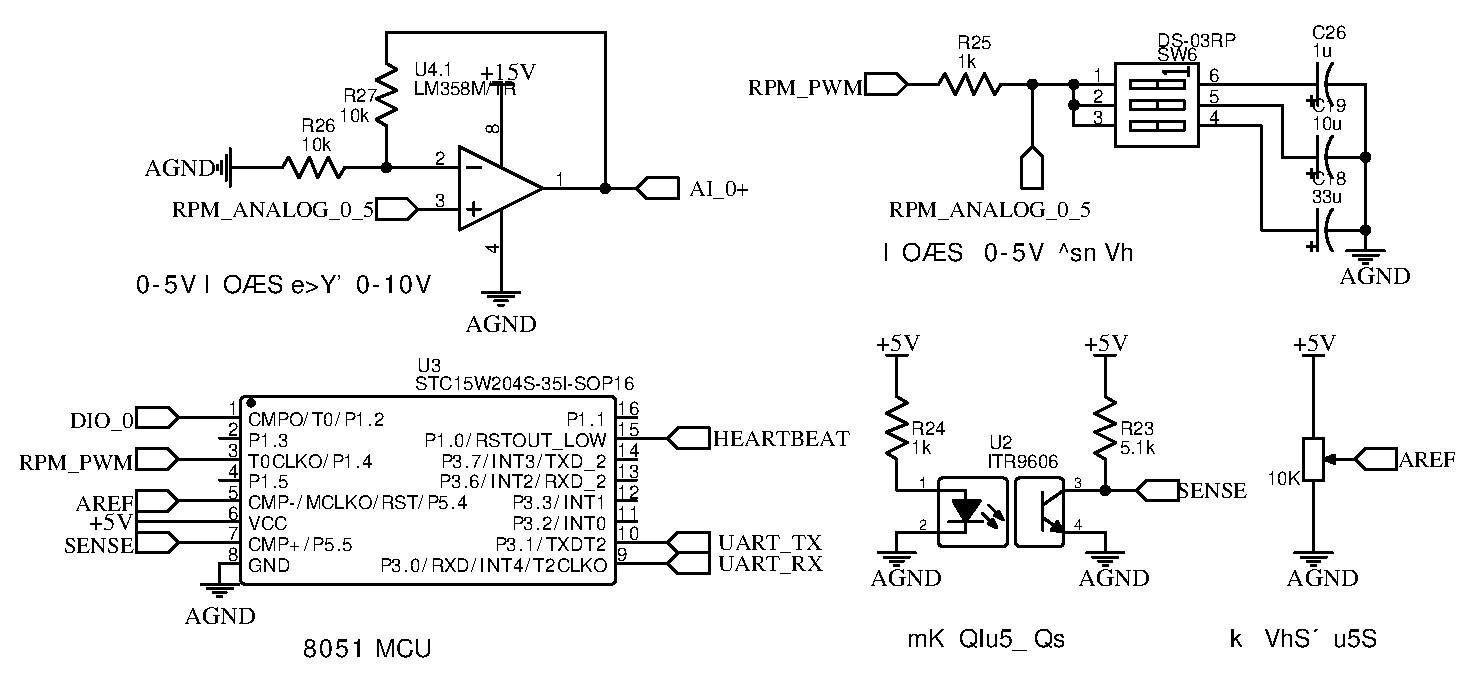
\includegraphics[width=14cm]{./figs/speed_measure_sch.pdf}
  \caption{光电转速测量电路原理图}\label{speed_measure_sch}
\end{figure}

直流电机通过专用支架安装在实验板上,其输出轴上带有12孔的码盘,码盘的打孔区位于ITR9606型红外光电传感器的槽中。电机每旋转一周,光电传感器将产生12个周期的高低电位信号。嵌入式微控制器U3内置一路模拟电压比较器,并可产生比较器中断。通过编写应用程序即可测出单位时间内光电传感器输出信号的周期数,进而测得电机转速。用于实现此功能的MCU程序已列于附录中。

MCU根据所测出的转速产生一路推挽输出模式的PWM信号,经RC电路平滑为直流电压后,被U4放大至2倍,形成范围为0--10V的转速电压信号。学生可根据需要选择不同大小的电容,决定电压信号的平滑程度。选择电容较小时转速信号响应迅速,但可在myDAQ端测出较大噪声。选择电容较大时可获得高信噪比的信号,同时也会引入延迟。

\subsection{电机驱动与电流采样电路}
图\ref{motor_mosfet_sch}为电机驱动与电流采样电路的原理图。Q2为Fairchild公司出品的8N60C型N沟道增强型MOSFET(可用其他型号N沟道增强型MOSFET替换,但需重新调节栅极电压增益)。
\begin{figure}[h!]\centering
  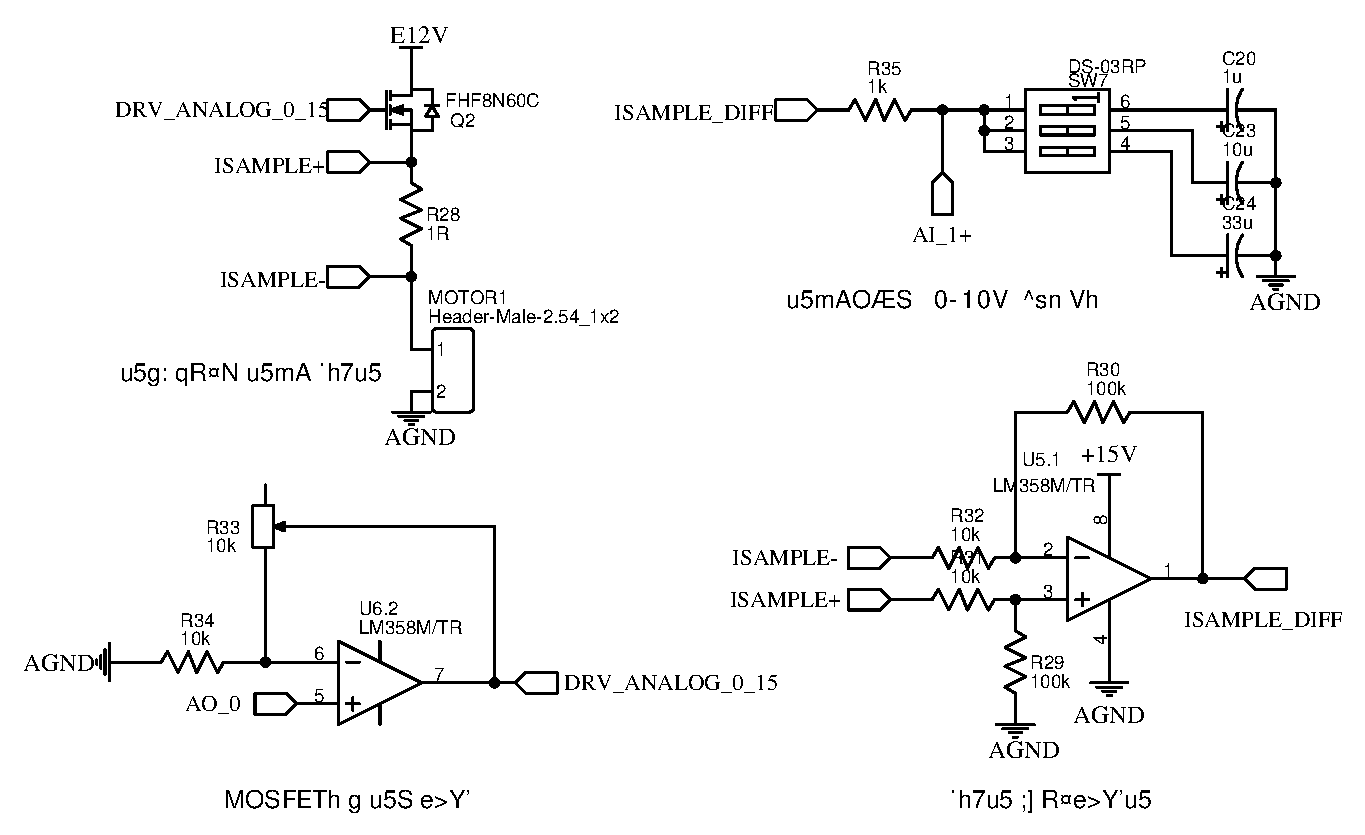
\includegraphics[width=14cm]{./figs/motor_mosfet_sch.pdf}
  \caption{电机驱动与电流采样电路原理图}\label{motor_mosfet_sch}
\end{figure}

myDAQ提供的0 -- 10V功率控制信号经U6.2放大输入Q2的栅极。调试电路时,运行提供的MATLAB程序手动给出10V控制信号,并调节R33使Q2临界达到饱和状态(电机转速临界增加到最大)。在该配置下,当myDAQ提供0 -- 10V信号时,Q2工作在可变电阻区,等效于将电阻$R_{DS}$串联在电机回路中,实现对电机的调速。

电机工作时,电流流过阻值为1$\Omega$的功率电阻R28,其两端产生与电流线性相关的电势差,经差动放大电路放大10倍后送至myDAQ的模拟输入端。此时1A电流对应10V电压,即myDAQ的最大测量范围。经过测试,电机两端电压12V的条件下发生堵转时,电流不超过0.8A,故此测量范围适合进行实验。

\subsection{实验板卡PCB设计}
图\ref{motor_board}为直流电机调速实验的PCB设计图。学生除可观察电机运转状态外,还可控制MCU内置电压比较器的比较阈值,观察比较结果,设置电压信号RC滤波器的平滑程度,以及观察频率测量程序的运行情况。
\begin{figure}[h!]\centering
  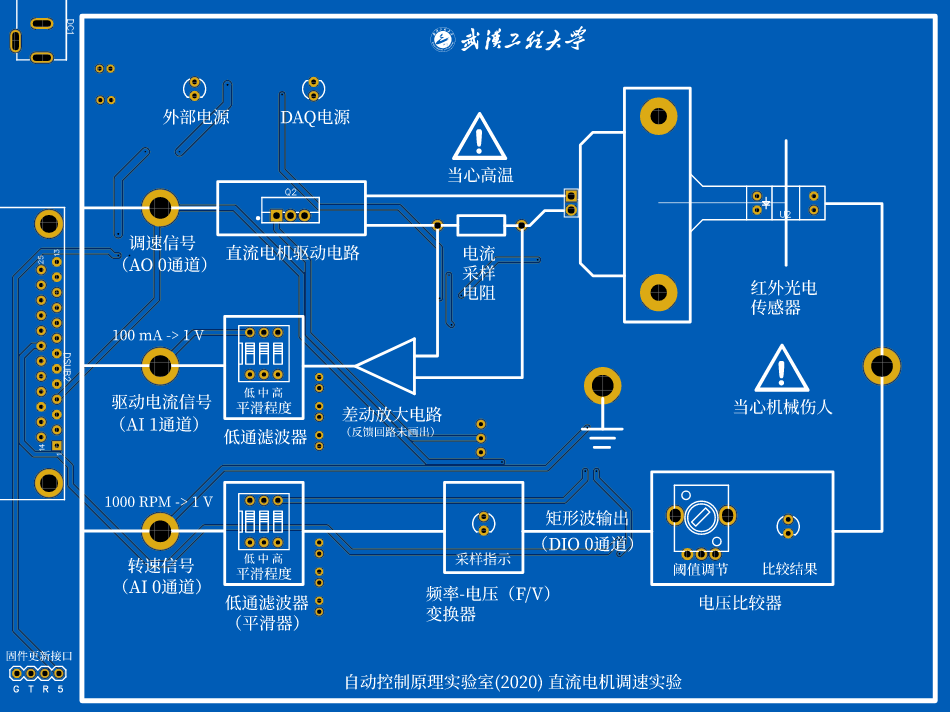
\includegraphics[width=14cm]{./figs/motor_board.png}
  \caption{直流电机调速实验PCB设计图}\label{motor_board}
\end{figure}

myDAQ的电源输出总功率不可超过500mW。板卡上预留了一个12V外部电源输入接口(内正外负),用以为直流电机提供高功率驱动电源。

\subsection{Simulink实验模型示例}
\begin{figure}[h!]\centering
  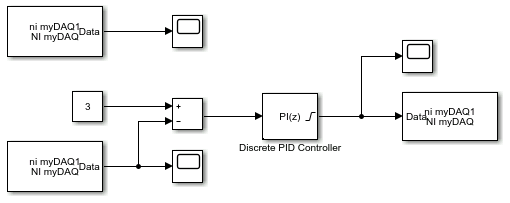
\includegraphics[width=12cm]{./figs/motor_pi.png}
  \caption{直流电机调速实验Simulink模型示例}\label{motor_pi}
\end{figure}
\begin{figure}[h!]\centering
  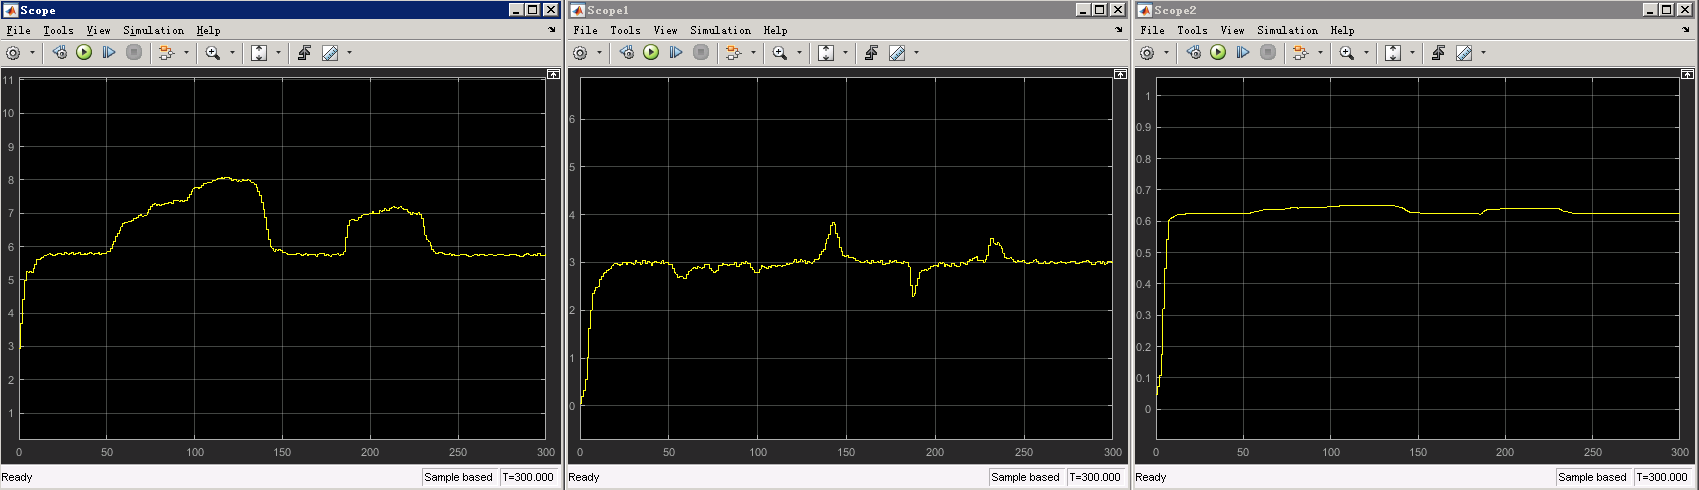
\includegraphics[width=16cm]{./figs/motor_result.png}
  \caption{直流电机调速实验Simulink运行结果}\label{motor_result}
\end{figure}

\section{温度控制实验}

\subsection{设计目的}
板卡上设计了温度测量,加热器与风扇驱动电路,以及一个大型金属功率电阻作为被控对象,用于进行温度闭环控制实验。myDAQ输出一个0--10V的模拟电压信号来控制加热器驱动电路中PWM的占空比,实现对加热器功率的调节。板上设计有AD590温度测量集成电路,其信号经过运算放大器变换成0--10V模拟电压送至myDAQ的模拟输入通道,对应的测量范围为0--100 ℃。学生可在Simulink环境中编写控制器来使被控对象(功率电阻)的温度稳定在某一设定值,也可开启风扇来调节被控对象的散热功率,以测试控制器的控制效果。

\subsection{PWM生成与加热器驱动电路}
在上一节介绍的电机调速实验中,MOSFET工作在线性区实现电机调速。经过实测,电机的平均电流在0.2 -- 0.5A之间,只要不出现长时间堵转的情况,不会造成MOSFET严重发热。在本实验中,加热器电流可达1A,需要采用PWM驱动的方式,使MOSFET仅工作在饱和和截止区,避免MOSFET发热。图\ref{temp_pwm_sch}为PWM生成电路与加热器驱动电路的原理图。
\begin{figure}[h!]\centering
  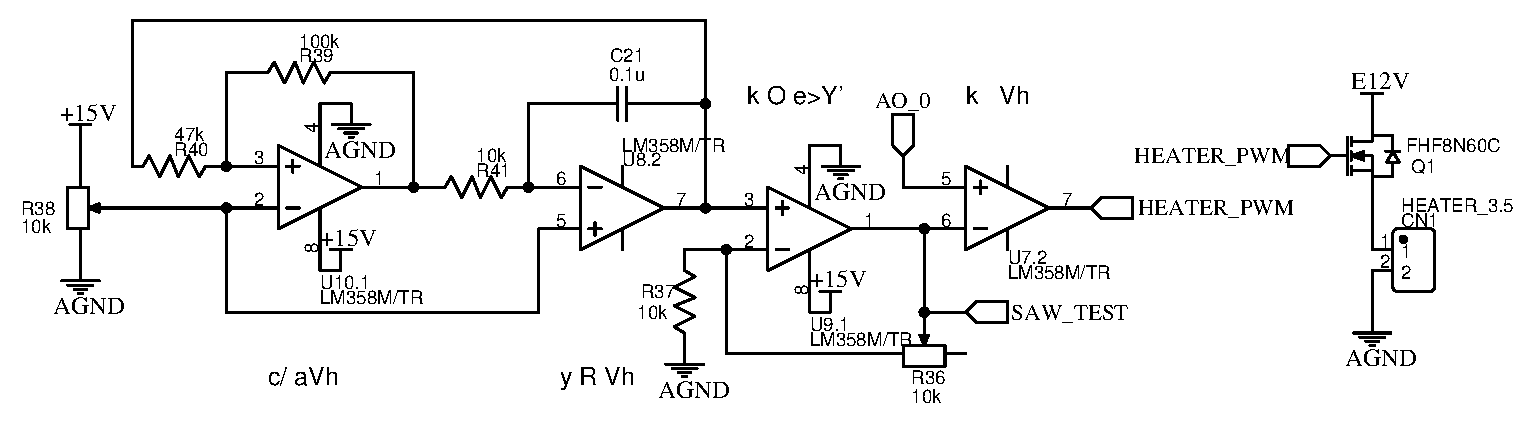
\includegraphics[width=14cm]{./figs/temp_pwm_sch.pdf}
  \caption{PWM生成与加热器驱动电路原理图}\label{temp_pwm_sch}
\end{figure}

运放U10.1构成自激振荡电路生成一定频率的方波,被运放U8.2积分后形成三角波。U9.1构成比例放大电路,将三角波的振幅调整至0 -- 10 V。U7.2以开环方式工作,作为电压比较器,将来自myDAQ的模拟电压与三角波进行比较,输出PWM波。当来自myDAQ的电压变化时,PWM的占空比相应变化,myDAQ的最大输出电压10V使PWM波的占空比为100\%,即恒为高电平,加热器以最大功率加热。

\subsection{温度测量电路}
图\ref{ad590_sch}为温度测量电路的原理图。U12为ADI公司出品的AD590型双端温度变送器,其输出电流信号与绝对温度成比例,每开尔文(K)对应电流1$\mu$A。R46为电流采样电阻。
\begin{figure}[h!]\centering
  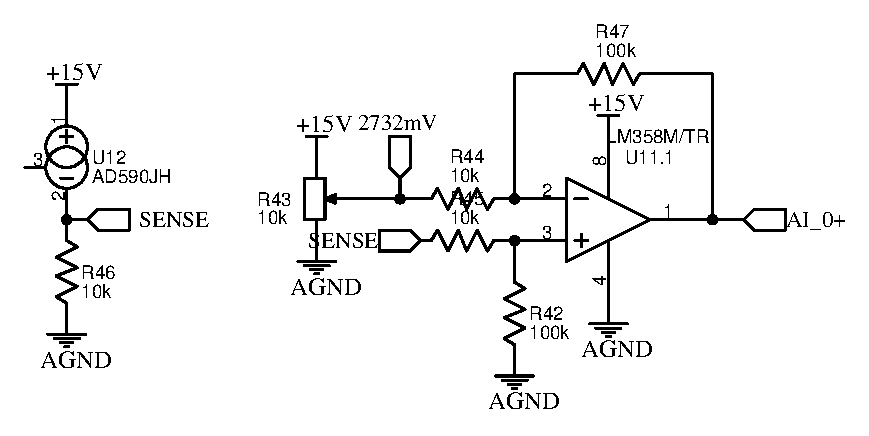
\includegraphics[width=9cm]{./figs/temp_ad590_sch.pdf}
  \caption{温度测量电路原理图}\label{ad590_sch}
\end{figure}

R46上的电压被U11.1构成的差动放大器减去2732mV(对应0℃与绝对零度-273℃的温差),并放大至10倍,得到代表温度的电压。0℃为0V,100℃为10V(myDAQ的最大测量范围)。

\subsection{散热风扇控制电路}
图\ref{temp_fan_sch}为散热风扇控制电路。U14为817C型光电耦合器,K1为松乐公司出品的SRS-05VDC型电磁继电器。
\begin{figure}[h!]\centering
  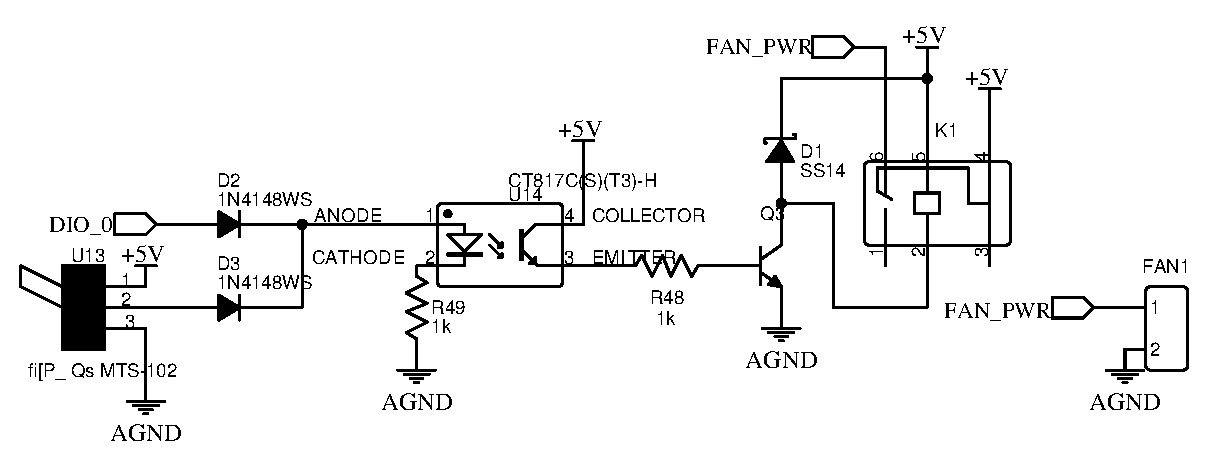
\includegraphics[width=13cm]{./figs/temp_fan_sch.pdf}
  \caption{散热风扇控制电路原理图}\label{temp_fan_sch}
\end{figure}

FAN1为间距2.54mm的插座,用于连接5V 0.12A无刷风扇。钮子开关U13为散热风扇强制启动开关,便于学生随时调整系统散热功率或使受控对象快速降温。二极管D2,D3构成或门,myDAQ的数字输出或钮子开关中的任意一个为高电平,即启动风扇。

\subsection{实验板卡PCB设计}
图\ref{temp_board}为温度控制实验的PCB设计图。学生可观察被控对象的状态,以及加热器、风扇的运行状态。
\begin{figure}[h!]\centering
  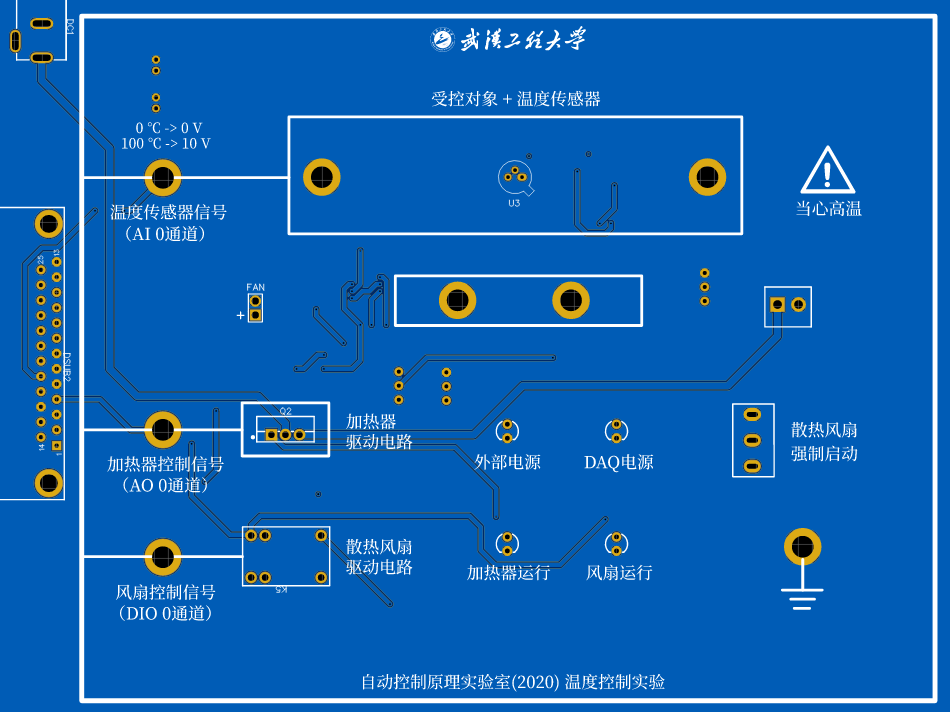
\includegraphics[width=14cm]{./figs/temp_board.png}
  \caption{温度控制实验PCB设计图}\label{temp_board}
\end{figure}

\begin{appendices}
  \section{8051 MCU电机测速固件}
  程序需使用Realview Keil A51汇编器编译,使用STC-ISP下载固件时需选择内部PLL时钟频率为35MHz。
  \lstinputlisting{../直流电机调速实验/MCU固件/f2pwm.a51}

\end{appendices}

\end{document}
